
\section{扎里斯基切空间}

我们从一个\trScheme{}在一点处的\trTangentSpace{}的定义开始。在那些「\trSmooth」的点处，它的表现一如你所熟知并且喜爱的那个\trTangentSpace；但它在其他的点处也照样有意义。换句话说，「\trSmooth」点处的几何直觉引导着定义，而定义又引导着所有点处的代数，这转而让我们得以精炼自己的几何直觉。

这个定义很短，却出人意料。主要的困难在于让你自己相信：它配得上「\trTangentSpace」之名。这件事解释起来颇为棘手，因为我们想表明它与我们的直觉相合，而我们的直觉却比我们所以为的更糟。所以你现在只管接受这个定义，日后再让自己确信它是合理的。

\textbf{13.1.1.}\ \emph{\trhDefinition{}。}\quad 一个\trLocalRing{} $(A,\mathfrak{m})$ 的 \textbf{\trZariski{}\trCotangentSpace}（Zariski cotangent space）定义为 $\mathfrak{m}/\mathfrak{m}^2$；它是\trResidueField{} $A/\mathfrak{m}$ 上的一个\trVectorSpace。其对偶\trVectorSpace{}便是 \textbf{\trZariski{}\trTangentSpace}。若 $X$ 是一个\trScheme，则点 $\mathrm{p}\in X$ 处的 \textbf{\trZariski{}\trCotangentSpace} $\mathrm{T}^{\vee}_{X,\mathrm{p}}$ 定义为\trLocalRing{} $\OO_{X,\mathrm{p}}$ 的\trZariski{}\trCotangentSpace，\textbf{\trZariski{}\trTangentSpace} $\mathrm{T}_{X,\mathrm{p}}$ 与之相仿。（注意：对\emph{任意}\trRing{} $A$ 的\emph{任意}\trMaximalIdeal{} $\mathfrak{m}$，我们都\trCanonically{}有 $\mathfrak{m}/\mathfrak{m}^2=\mathfrak{m}A_{\mathfrak{m}}/\mathfrak{m}^2A_{\mathfrak{m}}$——请务必弄明白为什么。）\trZariski{}\trCotangentSpace{}的元素称为\textbf{\trCotangentVector}（cotangent vectors）或\textbf{\trDifferential}（differentials）；\trTangentSpace{}的元素则称为\textbf{\trTangentVector}（tangent vectors）。

比之\trTangentSpace，\trCotangentSpace{}在代数上更为自然——因为它的定义更短。这背后有一个道理上的缘由：\trCotangentSpace{}更自然地由「空间上的函数」所确定，而我们思考\trScheme{}的方式，恰恰是紧扣「其上的函数」。这一点日后还会出现。

下面给出两条论证，说明这个定义是合理的。希望其中一条能合你心意。

在\trDifferentialGeometry{}中，一点处的\trTangentSpace{}有时被定义为在该点处的诸\trDerivation（derivation）组成的\trVectorSpace。一个流形在点 $\mathrm{p}$ 处的\trDerivation，是一个 $\mathbb{R}$-线性运算：它取 $\mathrm{p}$ 附近的函数 $f$（即 $\OO_{\mathrm{p}}$ 的元素）为输入，输出 $\mathbb{R}$ 中的元素 $f'(\mathrm{p})$，并且满足\trLeibniz{}法则（Leibniz rule）
\[
(fg)'=f'g+g'f.
\]
（我们日后将在更一般的设定下定义\trDerivation，见 \S21.2.17。）一个\trDerivation{}无非是一个映射 $\mathfrak{m}\to\mathbb{R}$，其中 $\mathfrak{m}$ 是 $\OO_{\mathrm{p}}$ 的\trMaximalIdeal。（映射 $\OO_{\mathrm{p}}\to\mathbb{R}$ 经由映射 $\OO_{\mathrm{p}}\to\mathfrak{m}$、$f\mapsto f-f(\mathrm{p})$ 延拓了这件事。）但 $\mathfrak{m}^2$ 被映到 $0$：因为若 $f(\mathrm{p})=g(\mathrm{p})=0$，则
\[
(fg)'(\mathrm{p})=f'(\mathrm{p})g(\mathrm{p})+g'(\mathrm{p})f(\mathrm{p})=0.
\]
于是，一个\trDerivation{}诱导出映射 $\mathfrak{m}/\mathfrak{m}^2\to\mathbb{R}$，也就是说，$(\mathfrak{m}/\mathfrak{m}^2)^{\vee}$ 的一个元素。

\textbf{13.1.A.（练习）}\quad 检验这件事是可逆的，也就是说：任何线性映射 $\mathfrak{m}/\mathfrak{m}^2\to\mathbb{R}$ 都给出一个\trDerivation。换言之，验证\trLeibniz{}法则成立。

这里还有第二条更模糊的动机，说明这个定义对 $\mathbb{A}^n$ 的原点处的\trCotangentSpace{}是合理的。（我更喜欢这一条，因为它更原始、更初等。）$\mathbb{A}^n$ 上的函数应当限制成\trTangentSpace{}上的一个线性函数。$x^2+xy+x+y$ 「在原点附近」限制出怎样的（线性）函数？你自然会答：$x+y$。于是我们「挑出线性项」。从而 $\mathfrak{m}/\mathfrak{m}^2$ 恰是\trTangentSpace{}上的那些线性泛函，故 $\mathfrak{m}/\mathfrak{m}^2$ 就是\trCotangentSpace。特别地，你应当把在一个点处消失的函数（即落在 $\mathfrak{m}$ 中的那些）想象成以上述这个显然的方式给出\trTangentSpace{}上的函数。

\textbf{13.1.2.}\ \emph{老式例子。}\quad 计算\trZariski{}\trTangentSpace{}其实是件相当可以亲手操作的事，因为你可以完全像当年学多元微积分时那样把它算出来。在 $\mathbb{A}^3$ 中，我们有一条由 $x+y+z^2+xyz=0$ 与 $x-2y+z+x^2y^2z^3=0$ 切出的\trCurve。（你可以用\trKrull{}\trPrincipalIdealTheorem~12.3.3 来验证这是一条\trCurve，但不验证也不要紧。）原点附近的\trTangentLine{}是什么？（它在那里甚至\trSmooth{}吗？）答：第一张\trSurface{}看上去像 $x+y=0$，而第二张\trSurface{}看上去像 $x-2y+z=0$。这条\trCurve{}的\trTangentLine{}由 $x+y=0$ 与 $x-2y+z=0$ 切出。它是\trSmooth{}的（在传统意义下）。在多元微积分里，学生们要费好大的劲才能得到答案，因为我们不被允许教他们径直挑出线性项。

让我们把正在使用的这条事实明说出来。若 $A$ 是一个\trRing，$\mathfrak{m}$ 是一个\trMaximalIdeal，而 $f\in\mathfrak{m}$ 是在点 $[\mathfrak{m}]\in\Spec A$ 处消失的一个函数，那么 $\Spec A/(f)$ 在 $\mathfrak{m}$ 处的\trZariski{}\trTangentSpace，便由唯一一条线性方程 $f\pmod{\mathfrak{m}^2}$ 从 $\Spec A$ 的\trZariski{}\trTangentSpace（在 $\mathfrak{m}$ 处）中切出。下一道练习将逼你把这件事想透。

\textbf{13.1.B.（重要练习：「\trTangentSpace{}的\trKrull{}\trPrincipalIdealTheorem」——但比\trKrull{}\trPrincipalIdealTheorem~12.3.3 容易得多！）}\quad 设 $A$ 是一个\trRing，$\mathfrak{m}$ 是一个\trMaximalIdeal。若 $f\in\mathfrak{m}$，证明：$A/f$ 的\trZariski{}\trTangentSpace{}由 $f\pmod{\mathfrak{m}^2}$ 从 $A$ 的\trZariski{}\trTangentSpace{}中切出。（注意：我们可以先对 $f$ 取商、再在 $\mathfrak{m}$ 处取\trLocalization，也可以反着来，因为取商与取\trLocalization{}交换，\eqref{eq:localize-quotient-diagram}。）于是，$\Spec A/(f)$ 在 $[\mathfrak{m}]$ 处的\trZariski{}\trTangentSpace{}的\trDimension，要么等于 $\Spec A$ 在 $[\mathfrak{m}]$ 处的\trZariski{}\trTangentSpace{}的\trDimension，要么比它小一。（若\trDimension{}无穷，最后这句话应当被合适地解读，尽管这种情形没什么意思。）

这里再举一个例子来观察这条原理的实际作用，它拓广了例~13.1.2：$x+y+z^2=0$ 与 $x+y+x^2+y^4+z^5=0$ 切出一条\trCurve，它显然穿过原点。如果我请我教多元微积分的学生们计算这条\trCurve{}在原点处的\trTangentLine，他们会做一番计算，而那些计算归根结底（在他们不自知的情况下）正是在挑出线性项。他们最终会得到 $x+y=0$ 与 $x+y=0$ 这两条方程，而它们切出的是一张平面，不是一条直线。他们会感到不安，而我则会解释说：这是因为这条\trCurve{}在一个点处不\trSmooth，他们的技术不管用了。我们呢，则勇敢地宣布：\trTangentSpace{}就是由 $x+y=0$ 切出的，并且（很快就会）把这种病理用作「使一点成为奇点（或不\trRegular）」的定义。（直观地说，这条\trCurve{}在原点附近非常贴近于躺在平面 $x+y=0$ 之中。）注意：余切空间的\trDimension{}是从它「本该在」的位置向上跳的，而不是向下。（这绝非巧合：见定理~12.3.12。）

\textbf{13.1.C.（练习）}\quad 设 $Y$ 与 $Z$ 是 $X$ 的两个\trClosedSubscheme，二者都含有点 $\mathrm{p}\in X$。
\begin{enumerate}[label=(\alph*)]
\item 证明：$\mathrm{T}_{Z,\mathrm{p}}$ \trNatural{}地是 $\mathrm{T}_{X,\mathrm{p}}$ 的一个 $\kappa(\mathrm{p})$-子\trVectorSpace。
\item 证明：$\mathrm{T}_{Y\cap Z,\mathrm{p}}=\mathrm{T}_{Y,\mathrm{p}}\cap\mathrm{T}_{Z,\mathrm{p}}$。（左边的 $\cap$ 指\trSchemeTheoretic{}交。右边的 $\cap$ 指\trVectorSpace{} $\mathrm{T}_{X,\mathrm{p}}$ 的诸\trSubspace{}之交。）
\item 证明：$\mathrm{T}_{Y\cup Z,\mathrm{p}}$ 包含 $\mathrm{T}_{Y,\mathrm{p}}$ 与 $\mathrm{T}_{Z,\mathrm{p}}$ 的张成，此处 $\cup$ 依本语境的惯例指\trSchemeTheoretic{}并。
\item 证明：$\mathrm{T}_{Y\cup Z,\mathrm{p}}$ 可以严格大于 $\mathrm{T}_{Y,\mathrm{p}}$ 与 $\mathrm{T}_{Z,\mathrm{p}}$ 的张成。（提示：\cref{fig:scheme-theoretic-intersection}。）
\end{enumerate}

下面是\trZariski{}\trTangentSpace{}这一观念的一个令人愉悦的推论。

\textbf{13.1.3.}\ \emph{问题。}\quad 考虑\trRing{} $A=k[x,y,z]/(xy-z^2)$。证明：$(x,z)$ 不是\trPrincipalIdeal。

由于 $\dim A=2$（为什么？），而 $A/(x,z)\cong k[y]$ 具有\trDimension{} $1$，我们看到这个\trIdeal{}的\trCodimension{}为 $1$（因为对不可约\trVariety{}而言，\trCodimension{}是\trDimension{}之差，定理~12.2.9）。我们的几何图像是：$\Spec A$ 是一张\trCone（当 $\operatorname{char}k\neq2$ 时——见\mbox{练习~5.4.J}——我们可以把这\trQuadricSurface{}对角化为 $xy-z^2=\bigl((x+y)/2\bigr)^2-\bigl((x-y)/2\bigr)^2-z^2$），而 $(x,z)$ 是这张\trCone{}上的一条直线。（草图见\cref{fig:cone-line-xyz}。）这提示我们去考察这个锥点。

\begin{figure}[htbp]
\centering
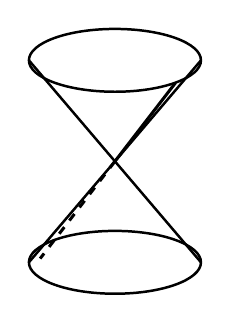
\begin{tikzpicture}[scale=0.95,line width=0.9pt]
  \draw (0,1.35) ellipse (1.15 and 0.42);
  \draw (0,-1.35) ellipse (1.15 and 0.42);
  \draw (-1.15,1.35) -- (0,0) -- (-1.15,-1.35);
  \draw (1.15,1.35) -- (0,0) -- (1.15,-1.35);
  \draw[line width=1.1pt] (0.81,1.05) -- (0,0);
  \draw[line width=1.1pt,dashed] (0,0) -- (-1.00,-1.30);
\end{tikzpicture}
\caption{$V(x,z)\subset\Spec k[x,y,z]/(xy-z^2)$ 是一张\trCone{}上的直线。（依原书手绘图重绘。）}\label{fig:cone-line-xyz}
\end{figure}

\textbf{13.1.4.}\ \emph{解答。}\quad 设 $\mathfrak{m}=(x,y,z)$ 是对应于原点的\trMaximalIdeal。于是 $\Spec A$ 在原点处的\trZariski{}\trTangentSpace{}具有\trDimension{} $3$，而 $\Spec A/(x,z)$ 在原点处的\trZariski{}\trTangentSpace{}具有\trDimension{} $1$。但由\mbox{练习~13.1.B}，$\Spec A/(f)$ 在原点处的\trZariski{}\trTangentSpace{}必定具有至少为 $2$ 的\trDimension。（附赠的收获是：我们顺便证明了 $A$ 不是\trUFD，依据是引理~12.1.7。\footnote{原书此处作（by Lemma 12.1.7.))），末尾衍一右括号，径删。——译者注}）

\textbf{13.1.5.}\ \hard\ \emph{\trhRemark{}。}\quad 解这道题还有另一条路，它不依赖\trZariski{}\trTangentSpace{}的定义：利用这个环是\trGrading{}的这一事实（其中 $x$、$y$、$z$ 的次数都是 $1$），且\trIdeal{} $(x,z)$ 是\trHomogeneous{}理想。（你也许会乐于亲自把这件事想一遍。）使用\trTangentSpace{}的优越性在于：它也适用于没有\trGrading{}的更一般的情形。例如，(a) $(x,z)$ 不是 $k[x,y,z]/(xy-z^2-z^3)$ 的\trPrincipalIdeal。作为另一个例子，(b) $(x,z)$ 不是\trLocalRing{} $(k[x,y,z]/(xy-z^2))_{(x,y,z)}$（「这张\trCone{}的\trGerm」）的\trPrincipalIdeal。然而我们提醒一句：分次情形仍然非常有用。把一个\trFiltered{}环换成其「\trAssociatedGraded」（associated graded）环的构造，可以把更一般的环变成\trGradedRing（并且可以用来把例子 (a) 化为分次情形）。\trCompletion{}的构造则可以把\trLocalRing{}变成\trGrading{}局部环（并且可以用来把例子 (b) 在本质上也化为分次情形）。\trFiltered{}环将在 \S13.9 中登场；\trAssociatedGraded{}构造将在我们讨论\trBlowup{}时（\S22.3）隐含地出现；而\trCompletion{}的诸多面向将在第 28 章中得到描述。

\textbf{13.1.D.（练习）}\quad 证明：$(x,z)\subset k[w,x,y,z]/(wz-xy)$ 是一个\trCodimension{}为 $1$ 却非\trPrincipalIdeal{}的\trIdeal，用的是解答~13.1.4 的方法。（这一情形的\trProjectivization{}——一张\trSmooth{}\trQuadricSurface{}上的一条直线——见\cref{fig:ruled-line-quadric}。）这个例子就是\mbox{练习~5.4.D}之后随即许诺的那一个。\mbox{练习~15.5.N}给出了一个改进：这个\trClosedSubset{} $x=z=0$ 甚至不是由单独一条方程\trSetTheoretic{}地切出的。

\begin{figure}[htbp]
\centering
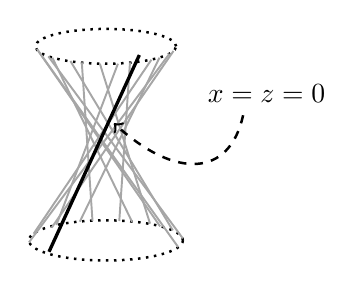
\begin{tikzpicture}[scale=0.85,line width=0.7pt]
  \draw[dotted,line width=0.9pt] (0,1.45) ellipse (1.05 and 0.26);
  \draw[dotted,line width=0.9pt] (0,-1.45) ellipse (1.15 and 0.30);
  \draw[gray!70] (-1.03,1.41) -- (1.08,-1.55);
  \draw[gray!70] (-0.86,1.30) -- (1.15,-1.42);
  \draw[gray!70] (-0.53,1.23) -- (1.00,-1.30);
  \draw[gray!70] (-0.09,1.19) -- (0.66,-1.20);
  \draw[gray!70] (0.36,1.21) -- (0.20,-1.16);
  \draw[gray!70] (0.80,1.28) -- (-0.39,-1.17);
  \draw[gray!70] (1.01,1.38) -- (-0.81,-1.26);
  \draw[gray!70] (-1.01,1.38) -- (0.81,-1.24);
  \draw[gray!70] (-0.80,1.28) -- (0.39,-1.17);
  \draw[gray!70] (-0.36,1.21) -- (-0.20,-1.16);
  \draw[gray!70] (0.18,1.19) -- (-0.74,-1.22);
  \draw[gray!70] (0.68,1.25) -- (-1.08,-1.35);
  \draw[gray!70] (0.95,1.34) -- (-1.15,-1.48);
  \draw[line width=1.2pt] (-0.85,-1.62) -- (0.50,1.32);
  \node at (2.40,0.75) {$x=z=0$};
  \draw[dashed,line width=0.9pt,->] (2.05,0.42) .. controls (1.85,-0.50) and (1.05,-0.55) .. (0.12,0.30);
\end{tikzpicture}
\caption{光滑\trQuadricSurface{} $V(wz-xy)\subset\mathbb{P}^3$ 上的直线 $V(x,z)$。（依原书手绘图重绘。）}\label{fig:ruled-line-quadric}
\end{figure}

\textbf{13.1.E.（练习）}\quad 设 $A=k[w,x,y,z]/(wz-xy)$。证明：$\Spec A$ 不是\trFactorial{}的。（\mbox{练习~5.4.L}表明 $A$ 不是\trUFD，但这还不够——为什么 $A$ 在素理想 $(w,x,y,z)$ 处的\trLocalization{}不是\trFactorial{}的？一种可能是「直接」做这件事，试着模仿\mbox{练习~5.4.L}的解法，但这很难。不如改用一条中间结果：在\trUFD{}中，任何\trCodimension{} $1$ 的\trPrimeIdeal{}都是\trPrincipalIdeal（引理~12.1.7），并结合\mbox{练习~13.1.D}来考虑。）由于当 $\operatorname{char}k\neq2$ 时 $A$ 是\trIntegrallyClosed{}的（\mbox{练习~5.4.I(c)}），这就给出了一个\trNormal{}却不\trFactorial{}的\trScheme{}的例子，正如\mbox{练习~5.4.F}所许诺的。稍作推广的版本将在\mbox{练习~22.4.N}中给出。

\textbf{13.1.F.（不甚重要的练习：「高阶数据」）}\quad （这个练习很有趣，但不会被用到。）
\begin{enumerate}[label=(\alph*)]
\item 在\mbox{练习~3.7.B}中，你计算过切出 $\mathbb{A}^3_k$ 的（并起来的）三条\trCoordinate{}轴的那些方程。（把这个\trScheme{}记作 $X$。）你的\trIdeal{}应当已经具有三个\trGenerator。证明：这个\trIdeal{}不能由更少的元素生成。（提示：模 $\mathfrak{m}=(x,y,z)$ 工作不会给出任何有用的信息，故请模 $\mathfrak{m}$ 的一个更高的幂工作。）
\item 证明：$\mathbb{A}^3_k$ 中的诸\trCoordinate{}轴到 $\mathbb{A}^3_k$ 中的嵌入并非\trRegularEmbedding。（这是 \S9.5 末尾所许诺的。）
\end{enumerate}

\textbf{13.1.6.}\ \emph{\trMorphism{}与\trTangentSpace。}\quad 设 $\pi\colon X\to Y$，且 $\pi(\mathrm{p})=\mathrm{q}$。假如我们身处可微流形的\trCategory，我们便会期待有一个切映射，从 $\mathrm{p}$ 的\trTangentSpace{}到 $\mathrm{q}$ 处的\trTangentSpace。事实也确实如此；我们有\trStalk{}的一个映射 $\OO_{Y,\mathrm{q}}\to\OO_{X,\mathrm{p}}$，它把前者的\trMaximalIdeal{} $\mathfrak{n}$ 送到后者的\trMaximalIdeal{} $\mathfrak{m}$（当我们简略地讨论\trLocallyRingedSpace{}时曾验证过这是一个「局部态射」；见 \S7.3.1）。于是 $\mathfrak{n}^2$ 被映到 $\mathfrak{m}^2$，由此我们见到 $\mathfrak{n}/\mathfrak{n}^2$ 被映到 $\mathfrak{m}/\mathfrak{m}^2$。若 $(\OO_{X,\mathrm{p}},\mathfrak{m})$ 与 $(\OO_{Y,\mathrm{q}},\mathfrak{n})$ 具有相同的\trResidueField{} $\kappa$，从而 $\mathfrak{n}/\mathfrak{n}^2\to\mathfrak{m}/\mathfrak{m}^2$ 是 $\kappa$-\trVectorSpace{}之间的一个线性映射，那么我们便有一个自然映射 $(\mathfrak{m}/\mathfrak{m}^2)^{\vee}\to(\mathfrak{n}/\mathfrak{n}^2)^{\vee}$。这就是我们所寻求的、从 $\mathrm{p}$ 的\trTangentSpace{}到 $\mathrm{q}$ 处的\trTangentSpace{}的映射。（旁注：注意\emph{余切}映射\emph{总是}存在，不要求 $\mathrm{p}$ 与 $\mathrm{q}$ 具有相同的\trResidueField——这正是一个信号，表明在\trAlgebraicGeometry{}中，\trCotangentSpace{}比\trTangentSpace{}更为自然。）

\textbf{13.1.G.（练习）}\quad 设 $X$ 是一个 $k$-\trScheme。描述从 $\Mor_k(\Spec k[\epsilon]/(\epsilon^2),X)$ 到如下数据的一个\trNatural{}\trBijection：一个具有\trResidueField{} $k$ 的点 $\mathrm{p}$（必是一个\trClosedPoint），以及 $\mathrm{p}$ 处的一个\trTangentVector。（这在例如形变理论（deformation theory）中很重要。我们不会用到它，所以你可以把它当作一件奇物。）

\textbf{13.1.H.（练习：好玩的算术操练）}\quad 求 $\mathbb{Z}[2i]\cong\mathbb{Z}[x]/(x^2+4)$ 中点 $[(2,2i)]$ 处\trZariski{}\trTangentSpace{}的\trDimension。再求 $\mathbb{Z}[\sqrt{-2}]\cong\mathbb{Z}[x]/(x^2+2)$ 中点 $[(2,x)]$ 处\trZariski{}\trTangentSpace{}的\trDimension。（若你更喜欢这些例子的几何版本，把 $\mathbb{Z}$ 换成 $\mathbb{C}$、把 $2$ 换成 $y$：考虑 $\mathbb{C}[x,y]/(x^2+y^2)$ 与 $\mathbb{C}[x,y]/(x^2+y)$。）

\textbf{13.1.7.\ 有限型情形下的一个重要诠释：\trJacobianMatrix{}\trCorank。}

\textbf{13.1.I.（重要练习：\trJacobianMatrix{}算出有理点处的\trZariski{}\trCotangentSpace）}\quad 设 $X$ 是一个\trFiniteType{} $k$-\trScheme。那么\trLocally{}地它形如 $\Spec k[x_1,\dots,x_n]/(f_1,\dots,f_r)$。证明：在一个 $k$-\trValuedPoint（即具有\trResidueField{} $k$ 的一个\trClosedPoint）处的\trZariski{}\trCotangentSpace，由「雅可比映射」（Jacobian map）$k^r\to k^n$ 的\trCokernel{}给出，而这个映射由 \textbf{\trJacobianMatrix}（Jacobian matrix）
\begin{equation*}\tag{13.1.7.1}\label{eq:jacobian-corank-matrix}
J=
\begin{pmatrix}
\dfrac{\partial f_1}{\partial x_1}(\mathrm{p}) & \cdots & \dfrac{\partial f_r}{\partial x_1}(\mathrm{p})\\
\vdots & \ddots & \vdots\\
\dfrac{\partial f_1}{\partial x_n}(\mathrm{p}) & \cdots & \dfrac{\partial f_r}{\partial x_n}(\mathrm{p})
\end{pmatrix}.
\end{equation*}
给出。（这把我们那道「$\mathbb{A}^3$ 中由几个方程切出一条\trCurve」的例子精确化了——在那里我们挑出了线性项；见例~13.1.2。）你可能会警觉：$\frac{\partial f}{\partial x_1}$ 究竟是什么\emph{意思}？你需要 $\delta$ 与 $\epsilon$ 吗？不需要！只需形式地定义导数即可，例如
\[
\frac{\partial}{\partial x_1}\bigl(x_1^2+x_1x_2+x_2^2\bigr)=2x_1+x_2.
\]
提示：先在 $\mathrm{p}$ 为原点时做这件事，并考虑线性项，正如例~13.1.2 与\mbox{练习~13.1.B}那样。至于一般情形，「把 $\mathrm{p}$ 平移到原点去」。

\textbf{13.1.8.}\ \emph{\trhRemark{}。}\quad 这条结果可以推广到\trResidueField{}在 $k$ 上\trSeparable{}的那些\trClosedPoint（特别地，若 $\operatorname{char}k=0$ 或 $k$ 有限，则可推广到\emph{全部}\trClosedPoint）；见注记~21.2.34。我们等到第 21 章才来证明这件事，并不意味着它必定如此复杂；一个更初等的证明是可能的。

\textbf{13.1.9.}\ \emph{\trhWarning{}。}\quad 在数学中更常见（但并不普遍）的做法，是把\trJacobianMatrix{}定义为 \eqref{eq:jacobian-corank-matrix} 的转置。

\textbf{13.1.J.（练习：\trJacobianMatrix{}的\trCorank{}不依赖于表述）}\quad 设 $A$ 是一个\trFinitelyGenerated{} $k$-\trAlgebra，由 $x_1,\dots,x_n$ 生成，其关系理想（ideal of relations）$I$ 由 $f_1,\dots,f_r$ 生成。设 $\mathrm{p}$ 是 $\Spec A$ 的一点。
\begin{enumerate}[label=(\alph*)]
\item 设 $g\in I$。证明：把 $g$ 的各偏导数组成的一列添到\trJacobianMatrix{} \eqref{eq:jacobian-corank-matrix} 上，不改变其在 $\mathrm{p}$ 处的\textbf{\trCorank}（corank）（即\trCokernel{}的\trDimension）。进而证明：\trJacobianMatrix{}在 $\mathrm{p}$ 处的\trCorank{}不依赖于 $I$ 的诸\trGenerator{}的选取。
\item 设 $q(x_1,\dots,x_n)$ 是 $k[x_1,\dots,x_n]$ 中的一个多项式。令 $h$ 为多项式 $y-q(x_1,\dots,x_n)\in k[x_1,\dots,x_n,y]$。证明：$(f_1,\dots,f_r,h)$ 关于变量 $(x_1,\dots,x_n,y)$ 的\trJacobianMatrix，在 $\mathrm{p}$ 处与 $(f_1,\dots,f_r)$ 关于 $(x_1,\dots,x_n)$ 的\trJacobianMatrix{}具有相同的\trCorank。进而证明：\trJacobianMatrix{}在 $\mathrm{p}$ 处的\trCorank{}不依赖于 $A$ 的诸\trGenerator{}的选取。
\end{enumerate}
于是，每个\trFiniteType{} $k$-\trScheme{} $X$ 都自带一个内蕴的「\textbf{\trJacobianMatrix{}\trCorank{}函数}」（Jacobian corank function），它从（$X$ 的\trUnderlyingSet{}）映到 $\mathbb{Z}^{\ge0}$，在 $X$ 的 $k$-\trValuedPoint{} $\mathrm{p}$ 处取值为 $\dim_\kappa\mathrm{T}_{X,\mathrm{p}}$。我们暂时把这个函数记作 $\mathrm{JC}\colon X\to\mathbb{Z}^{\ge0}$，尽管日后将会发现，它其实是\trDifferential{}的\trCoherentSheaf{} $\Omega_{X/\kappa}$ 的\trRank（\mbox{练习~21.2.E}）。

\textbf{13.1.K.（容易的练习）}\quad 证明：$\mathrm{JC}$ 是一个\trUpperSemicontinuous{}的函数。

\textbf{13.1.L.（练习）}\quad 证明：$\mathrm{JC}$ 在 $k$ 的\trFieldExtension{}之下保持。更精确地说，若 $X$ 是一个\trFiniteType{} $k$-\trScheme，$\ell/k$ 是一个\trFieldExtension，并且在\trBaseChange{}映射 $X\times_k\ell\to X$（$\mathrm{p}\mapsto\mathrm{q}$）之下，证明 $\mathrm{JC}(\mathrm{p})=\mathrm{JC}(\mathrm{q})$。

\textbf{13.1.M.（练习）}\quad 证明：对任意 $\mathrm{p}\in X$，$\mathrm{JC}(\mathrm{p})\ge\dim_X\mathrm{p}$。（此时 $X$ 必然在 $k$ 上\trFiniteType，但 $\mathrm{p}$ 不必是 $X$ 的\trClosedPoint。）$X$ 在 $\mathrm{p}$ 处的\trDimension，即 $\dim_X\mathrm{p}$，定义于\mbox{练习~12.2.K}。提示：先料理 $k=\overline{k}$ 的情形，在这里以诸\trClosedPoint{}为杠杆。然后再对一般的 $k$ 证明这条结果，办法是证明不等式两侧都在\trFieldExtension{}之下保持（\mbox{练习~13.1.L}与\mbox{练习~12.2.M}）。

\textbf{13.1.N.（练习：计算\trProjective{} $k$-\trScheme{}的\trJacobianMatrix{}\trCorank{}函数）}\quad 设 $X\subset\mathbb{P}^n_k$ 由\trHomogeneous{}多项式 $f_i\in k[x_0,\dots,x_n]$（$1\le i\le r$）切出。证明：$X$ 的\trJacobianMatrix{}\trCorank{}函数比「射影雅可比矩阵」（projective Jacobian matrix）的\trCorank{}恰小 $1$：
\begin{equation*}\tag{13.1.9.1}\label{eq:projective-jacobian-corank}
\mathrm{JC}(\mathrm{p})=\operatorname{corank}
\begin{pmatrix}
\dfrac{\partial f_1}{\partial x_0}(\mathrm{p}) & \cdots & \dfrac{\partial f_r}{\partial x_0}(\mathrm{p})\\
\vdots & \ddots & \vdots\\
\dfrac{\partial f_1}{\partial x_n}(\mathrm{p}) & \cdots & \dfrac{\partial f_r}{\partial x_n}(\mathrm{p})
\end{pmatrix}-1.
\end{equation*}
你必须设法让右端有意义，因为射影\trJacobianMatrix{}的元素并不是函数；这个\trCorank{}到底是什么意思呢？
